\chapter{Konwolucyjne sieci neuronowe}
Konwolucyjne sieci neuronowe (ang. Convolutional Neural Networks)

funkcja obrazowa;
splot;
filtr;
jądro;
warstwy konwolucyjne;
wartwy aktywacji neuronów;
warstwy FC;
Dropout;
Normalizacja;

FP, TP, FN, TN

\section{Zarys historyczny}
\section{Problem nadmiernego dopasowania}
\label{sec-overffiting}
-dropout
Kolejnym zabiegiem wykorzystywanym tym razem w celu polepszenia generalizacji klasyfikacji zbioru danych było użycie techniki dropout [Dropout].

Combining the predictions of many different models is a very successful way to reduce test errors
[1, 3], but it appears to be too expensive for big neural networks that already take several days
to train. There is, however, a very efficient version of model combination that only costs about a
factor of two during training. The recently-introduced technique, called “dropout” [10], consists
of setting to zero the output of each hidden neuron with probability 0.5. The neurons which are
“dropped out” in this way do not contribute to the forward pass and do not participate in backpropagation.
So every time an input is presented, the neural network samples a different architecture,
but all these architectures share weights. This technique reduces complex co-adaptations of neurons,
since a neuron cannot rely on the presence of particular other neurons. It is, therefore, forced to
learn more robust features that are useful in conjunction with many different random subsets of the
other neurons. At test time, we use all the neurons but multiply their outputs by 0.5, which is a
reasonable approximation to taking the geometric mean of the predictive distributions produced by
the exponentially-many dropout networks.
We use dropout in the first two fully-connected layers of Figure 2. Without dropout, our network exhibits
substantial overfitting. Dropout roughly doubles the number of iterations required to converge.

--data augmentation


-5 fold
\section{Problem redukcji wymiarowości}

\section{Przykłady współczesnych topologii}
\subsection{AlexNet}
\label{AlexNet}
Sieć AlexNet, której nazwa pochodzi od imienia głównego twórcy tej architektury Alexa Krizhevsky, zawiera blisko 60 milionów parametrów i 650 tysięcy neuronów. Architekturę zaprezentowano na Rys. \ref{AlexNetTopology}
\begin{figure}[h!]
	\centering
	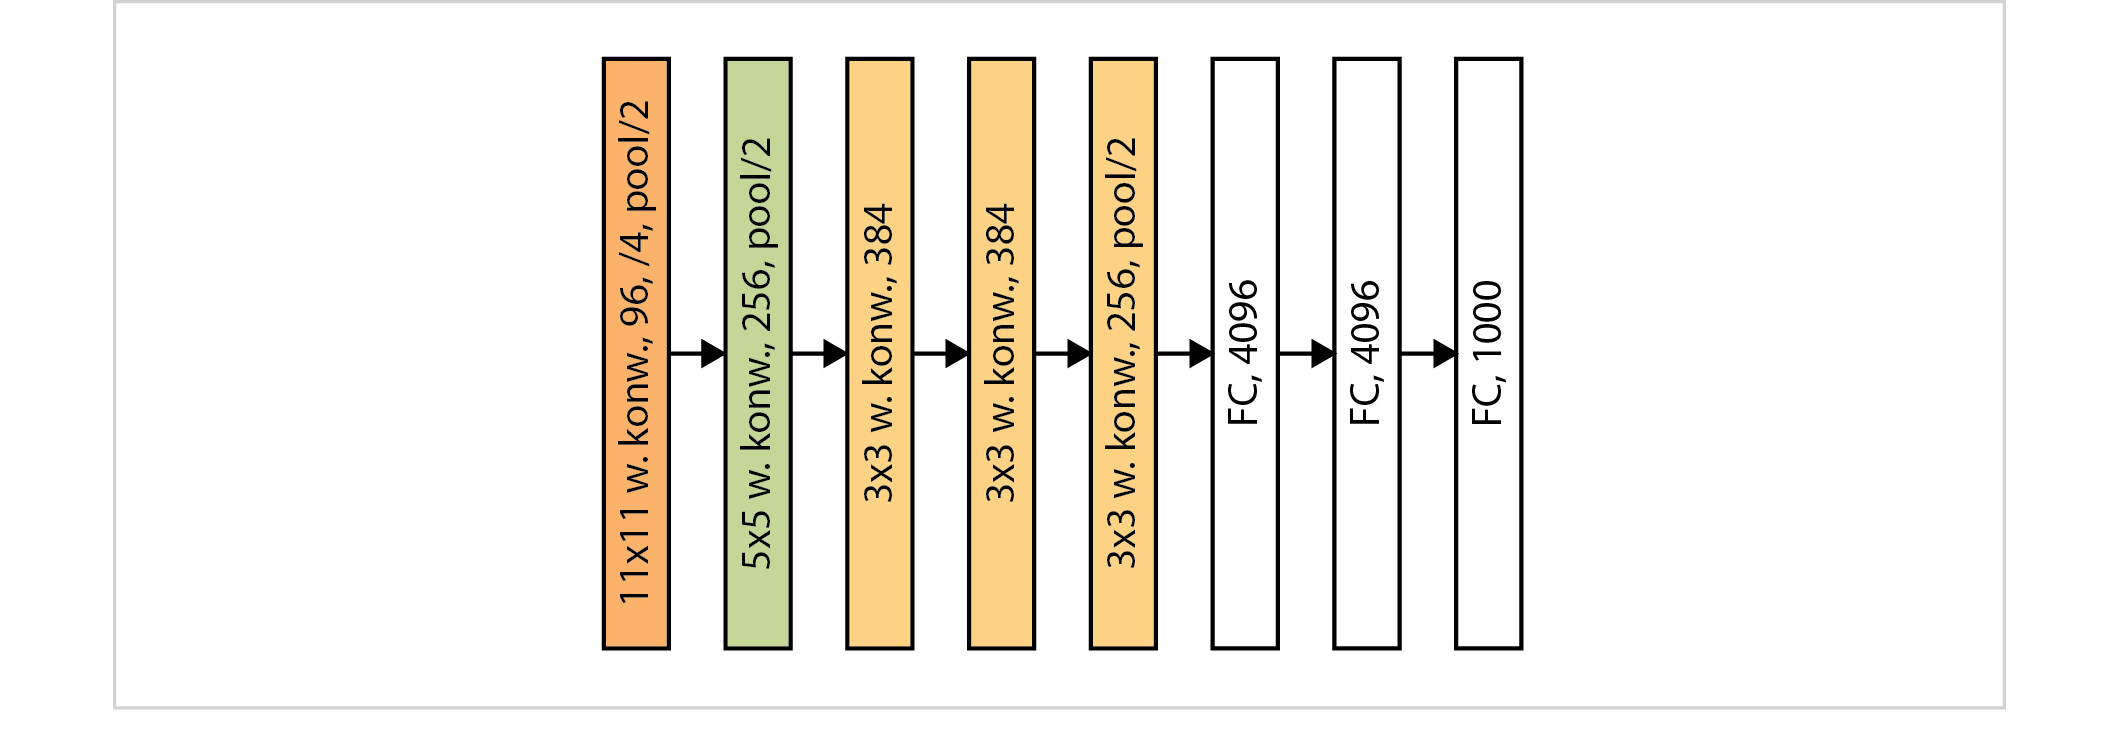
\includegraphics[width=0.55\textwidth]{figures/AlexNet.png}
	\caption{Topologia architektury AlexNet.}
	\label{AlexNetTopology}
\end{figure}

W skład topologii wchodzi pięć warstw konwolucyjnych i trzy typu fully-connected. Po pierwszej, drugiej i piątej warstwie konwolucyjnej występują operacje typu max-pool z jądrem o wymiarach 2$\times$2 \footnote{autorzy pracy podają też przykłady użycia jąder o wymiarze 2$\times$3, które nakładają się w przestrzeni funkcji obrazowej}. 

Pierwsza warstwa konwolucyjna przyjmuje na wejściu dane o wymiarze 227$\times$227$\times$3, na których wykonywana jest operacja splotu z 96 filtrami z jądrem splotu o wymiarach 11$\times$11$\times$3 i krokiem 4. W rezultacie (uwzględniając również operację max-pool) objętość wynikowa przekazywana do kolejnej warstwy ma wymiar 27$\times$27$\times$96. W drugiej warstwie konwolucyjnej wykonywana jest operacja splotu z 256 filtrami z jądrem o wymiarach 5$\times$5$\times$96. Wymiar objętości wynikowej zostaje ponownie zredukowany poprzez operacje max-pool do 13$\times$13$\times$256. Kolejne 3 warstwy konwolucyjne są połączone bezpośrednio ze sobą. Trzecia warstwa zawieraja 384 filtry o wymiarze 3$\times$3$\times$256, w skład czwartej wchodzą 384 filtry o wymiarze 3$\times$3$\times$384, a w piątej znajdują się 256 filtry ponownie o wymiarze 3$\times$3$\times$384. Końcowe dwie warstwy typu FC zawierają po 4096 neuronów, a ostatnia zawiera tyle neuronów ile klas występuje w ostatecznym podziale - w oryginalnej pracy było to 1000 [AlexNet].

W celu lepszego zrozumienia przetwarzania sygnału wejściowego przez sieć poniżej przedstawiono przykład algorytmu wykorzystywanego dla pierwszej warstwy konwolucyjnej opisywanej topologii: 
\begin{enumerate}
\item Z danych wejściowych o wymiarze [227$\times$227$\times$3] wybierany jest co czwarty blok (zarówno wzdłuż wysokości jak i szerokości) o wymiarach [11$\times$11$\times$3]. Punkty krawędziowe, które stanowią margines potrzebny do wyliczenia splotu są zazwyczaj pomijane. W rezultacie otrzymywanych jest 217 punktów w każdym rzędzie i w kolumnie, w których mieści się [55$\times$55] tj. 3025 bloków.
\item Zarówno 11$\times$11$\times$3 = 363 wagi znajdujące się w 96 filtrach jak i wartości 363 punktów obrazowych znajdujących sie 3025 blokach są przedstawiane w postaci macierzy $A$ o wymiarach [96$\times$363] i $B$ o wymiarach [363$\times$3025].
\item liczony jest iloczyn skalarny w postaci A$^\intercal$B = $C$, gdzie nowa, wyjściowa macierz $C$ ma wymiar [96$\times$3025].
\item Resultat w postaci macierzy $C$ ponownie przewymiarowywany jest na postać [55$\times$55$\times$96].  
\end{enumerate} 

W architekturze jako funkcję aktywacji neuronów wykorzystano ReLU, co znacząco przyspieszyło trening sieci. Dla przykładu uzyskano 6-krotne przyspieszenie treningu dla danych CIFAR-10 [CIFAR] w stosunku do tej samej topologii wykorzystującej funkcję aktywacji tanh.

Ponieważ funkcja ReLU nie posiada górnego ograniczenia neurony teoretycznie mogą posiadać nieograniczone wartości funkcji aktywacji. W celu polepszenia kontrastu pomiędzy neuronami i wydobycia tych, które na tle innych się wyróżniają, zastosowano normalizację:
\begin{equation}
b^i_{x,y} = a^i_{x,y}/\left ( k + \alpha \sum_{j=max(0,i-n/2)}^{min(N-1,i+n/2)} (a^i_{x,y})^2 \right  )^\beta 
\label{AlexNetNorm}
\end{equation}
gdzie $n$ to liczba filtrów znajdujących się w tej samej przestrzennej lokalizacji, $N$ to suma wszystkich filtrów w warstwie, $a^i_{x,y}$ to wartość funkcji aktywacji neuronu po splocie funkcji obrazowej na pozycji ($x$, $y$) z filtrem $i$, a $b$ to wynik normalizacji. Po zastosowaniu tej techniki autorom pracy udało się zredukować błąd klasyfikacji top-5 o wartość 1,2 punkta procentowego.

W kontekście zwiększenia efektywności treningu zastosowano powiększenie rozmiaru danych poprzez rotacje i modyfikacje funkcji obrazowej z wykorzystaniem czynników głównych (zob [AlexNet]), co zmniejszyło błąd top-1 o 1\%. Zastosowano również technikę dropout opisaną w \ref{sec-overffiting}. Ostatecznie wprowadzono także trening z wykorzystaniem wielu GPU (zob. Rys. \ref{AlexNetTopologyMultiGPU}). 

\begin{figure}[h!]
	\centering
	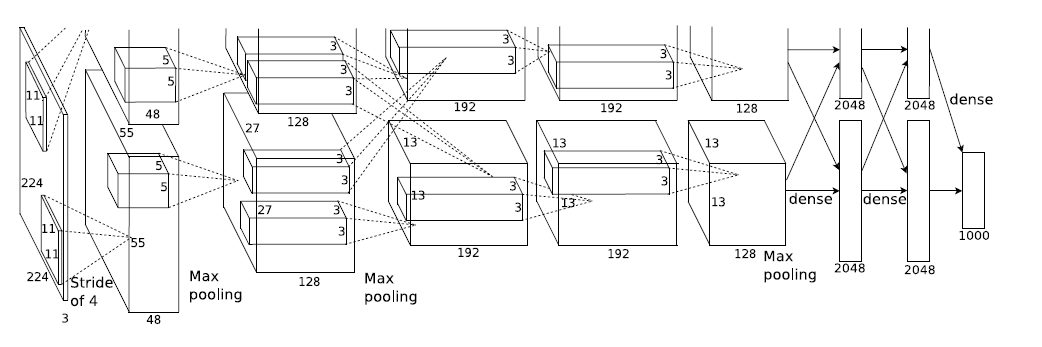
\includegraphics[width=0.8\textwidth]{figures/AlexNet-multiGPU.png}
	\caption{Topologia architektury AlexNet z podziałem na dwa akceleratory GPU.}
	\label{AlexNetTopologyMultiGPU}
\end{figure}

Topologia z podziałem na 2 karty zwiększyła dwukrotnie sumaryczną pamięć i pozwoliła na koalokację parametrów sieci.

Praca Alexa Krizhevsky, Ilya Sutskever i Geoffrey'a Hinton zapoczątkowała wzrost zainteresowania technikami głębokiego uczenia się, co doprowadziło do publikacji kolejnych podobnych architektur. Do najbardziej znanych należą ZFNet z 2013 roku [ZFNet], gdzie m.in. zastosowano zmniejszenie wymiaru jądra stosowanego w filtrach pierwszej warstwy konwolucyjnej do 7$\times$7 oraz VGGNet z 2014 roku, gdzie zastosowano większą liczbę warstw konwolucyjnych z mniejszym wymiarem jądra splotu. Innowacyjnym pomysłym, który został zaprezentowany również w 2014 było pojawienie się nowych modułów w sieci GoogleNet, która dokładniej została opisana w kolejnej podsekcji.

\subsection{GoogLeNet}

Architekturę o nazwie GoogLeNet zaprezentowano w 2014 r. w pracy [GoogleNet]. Nazwa architektury pochodzi od nazwy zwycięzkiego zespołu startującego w ILSVRC14, składającego się z pracowników firmy Google. Oryginalnie topologia składała się z 22 warstw i zawierała około 5 mln parametrów (12 razy mniej niż w przypadku sieci AlexNet). 

Redukcję liczby parametrów przy jednoczesnym podwyższeniu dokładności klasyfikacji i lokalizacji obiektów (zob. [ILSCV]) udało się uzyskać poprzez poszukiwania konstrukcji optymalnych lokalnych topologii i ich połączeń. Mianowicie, wiadomo że duża część funkcji aktywacji neuronów przyjmuje wartość 0 lub jest redundatna z powodu wysokiej korelacji między sobą (zob. [Arora z GoogleNet]). Matematyka dotycząca przetwarzania \textit{macierzy rzadkich}, tj. gdzie przeważająca liczba elementów przyjmuje wartość 0, jest dobrze znana np. [3-GoogleNet]. Jednak implementacje bibliotek do obliczeń związanych z algebrą liniową są zooptymalizowane pod kątem \textit{macierzy gęstych}, gdzie przeważająca liczba elementów przyjmuje wartości różne od 0 (zob. [16, 9 googleNet]). 

Ideą modułu incepcji zaproponowanego przez twórców GoogLeNet jest aproksymacja rzadkich macierzy z użyciem komponentów o gęstej strukturze. Takie komponenty nazwano \textit{modułami incepcji} (ang. \textit{inception modules}). Przykłądy modułów incepcji pokazano na Rys. \ref{GoogleNetInceptionModules} 
\begin{figure}[h!]
	\centering
	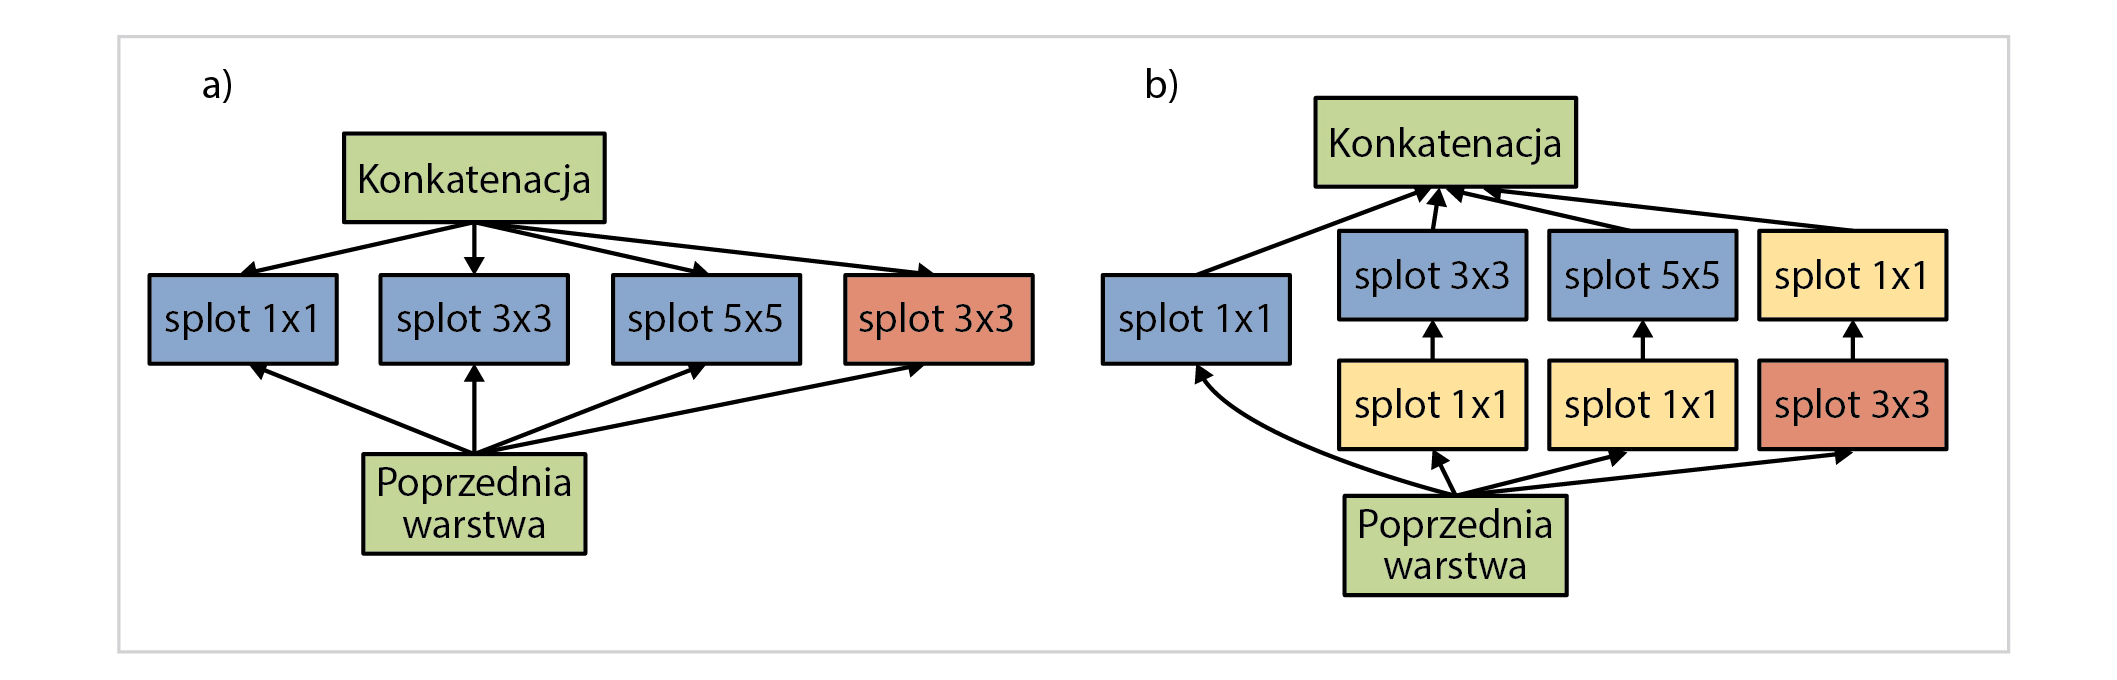
\includegraphics[width=0.8\textwidth]{figures/InceptionModules.png}
	\caption{Topologia architektury AlexNet z podziałem na dwa akceleratory GPU.}
	\label{GoogleNetInceptionModules}
\end{figure}

Rys. \ref{GoogleNetInceptionModules} (a) przedstawia najwną formę modułu incepcji, gdzie grupowane są operacje filtrów z jądrem o wymiarach 5$\times$5, 3$\times$3, 1$\times$1 oraz operacja max-pool. Rys. \ref{GoogleNetInceptionModules} (b) prezentuje koncepcję zooptymalizowaną obliczeniowo gdzie filtry 1$\times$1 służą do redukcji wymiarowości i używane są bezpośrednio przed splotami z bardziej wymagającymi obliczeniowo splotami z jądrami o wymiarach 5$\times$5 i 3$\times$3. 

Złożenie różnego rodzaju modułów dało topologię zaprezentowaną na Rys.
\begin{figure}[h!]
	\centering
	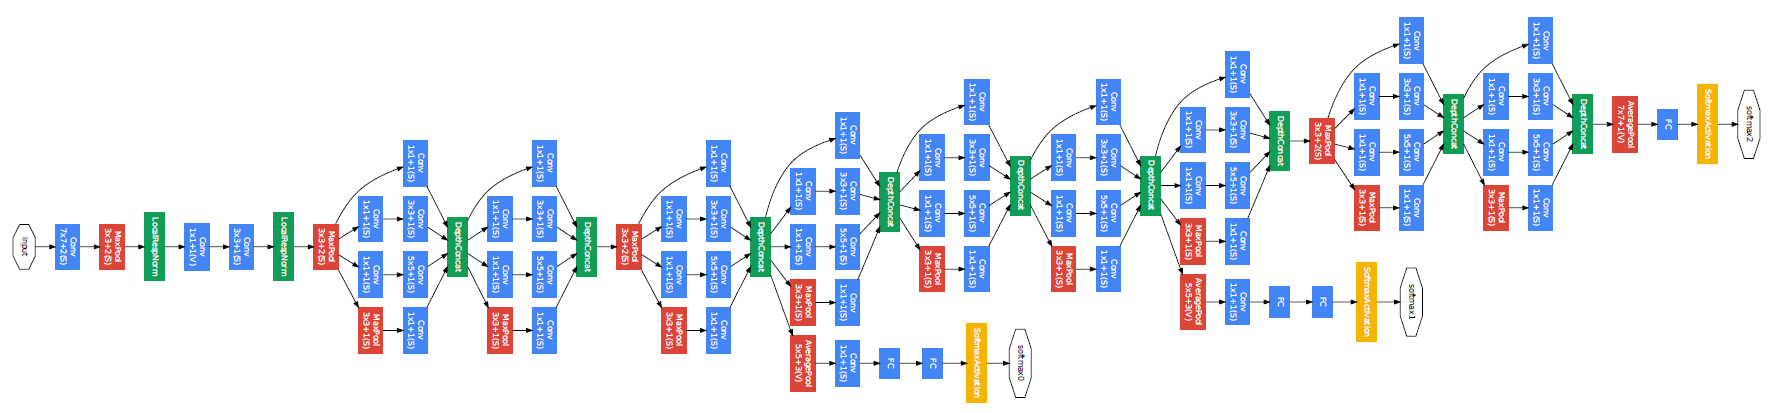
\includegraphics[width=1\textwidth]{figures/GoogleNet.png}
	\caption{Topologia architektury GoogleNet}
	\label{GoogleNetTopo}
\end{figure}

Dokładne zestawienie parametrów znajduje się w Tabeli \ref{GoogleNetParams}

\begin{table}[h!]
	\centering
	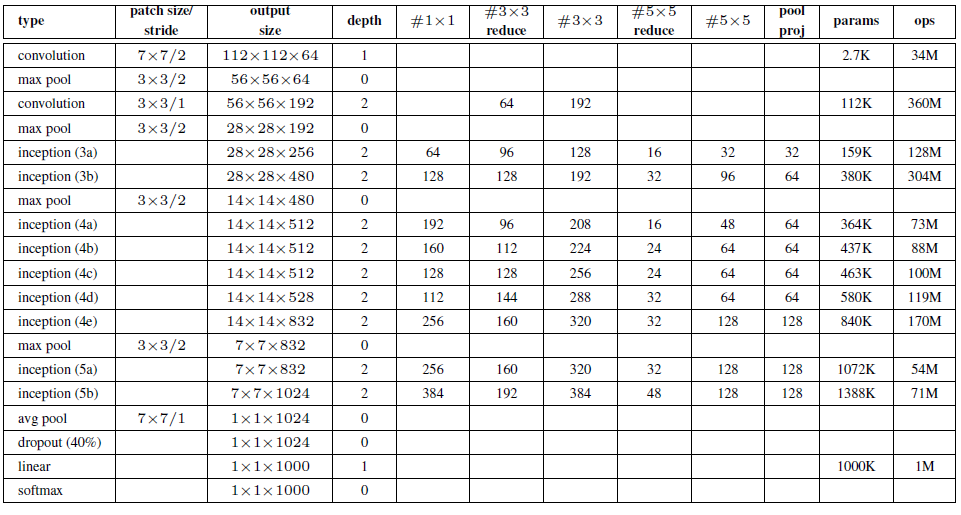
\includegraphics[width=1\textwidth]{figures/GoogleNetparams.png}
	\caption{Parametry architektury GoogleNet}
	\label{GoogleNetParams}
\end{table}

Ważną cechą sieci GoogleNet jest brak warstw typu FC na zakończeniu, gdzie w przypadku sieci AlexNet znajdowało się około 90\% parametrów. Końcowe wnioskowanie jest realizowane na podstawie wartości średniej z dwuwymiarowych map cech.

Dla lepszego zrozumienia idei redukcji wymiarowości realizowanej przez moduły incepcji, podobnie jak w przypadku sieci AlexNet, przeanalizowane zostanie działanie pierwszego modułu w topologii z Rys. \ref{GoogleNetTopo}.
Moduł zawiera 128 filtrów z jądrami o wymiarach 3$\times$3 i 32 filtry z jądrami o wymiarach 5$\times$5. Dane na wejściu modułu mają 192 kanały (zob. Tabela \ref{GoogleNetParams}). Dla przykładu, rząd wielkości obliczeń operacji splotów 32 filtrów 5$\times$5 wynosi 25$\times$32$\times$192=153 600 i dalej wzrastałby z głębokością sieci. W celu zapobiegnięcia nadmiarowi obliczeń stosowana jest redukcja z użyciem 16 filtrów z jądrem o wymiarach 1$\times$1. W efekcie rząd wielkości obliczeń spada do 16$\times$192 +  25$\times$32$\times$16=15 876, co pozwala na dalsze budowanie wielowarstwowych struktur.

Topologia GoogLeNet jest wciąż rozwijana. Po pierwszej prezentacji pojawiły się kolejne modernizacje wprowadzjące dodatkowe faktoryzacje modułów jak w Inception-v2 [Inception-v2], lub normalizacje wartości wynikowych poszczególnych warstw jak w Inception-v3 [Inception-v3]. Kolejny innowacyjny pomysł, bazujący na dodatkowych połączeniach między blokami, został wprowadzony w 2015 roku w sieci ResNet, która została opisana w kolejnej podsekcji.

\subsection{ResNet}

Jednym z najbardziej oczywistych pomysłów na polepszenie dokładności działania sieci neuronowych jest zwiększenie liczby warstw. Jednak wraz ze wzrostem liczby warstw, trening takich architektur z użyciem tradycyjnych metod gradientowych (takich jak algorytm wstecznej propagacji błędu) staje się mniej wydajny. Problem wynika z faktu, że zmiana wartości sygnału na wyjściu sieci w odpowiedzi na sygnał wejściowy jest mniejsza wraz ze wzrostem liczby warstw [ResNet]. W takiej sytuacji gradient wyliczany na podstawie sygnału będącego różnicą pomiędzy sygnałem wejściowym a wejściowym może przyjmować wartości bliskie 0 uniemożliwiając progres uczenia się. Problem zanikającego gradientu (ang. \textit{vanishing gradient problem}) rozwiązywany jest poprzez zastosowanie normalizacji oraz nieliniowych funkcji aktywacji, których przykłady zostały opisane w sekcji \ref{AlexNet} oraz szeroko w literaturze np. w [ResNet 2,3,4]. Dzięki tym mechanizmom algorytm treningu głębokich sieci neuronowych w większej liczbie przypadków zbiega do użytecznego minimum lokalnego. 

W momencie znalezienia takiego minimum dodanie kolejnych warstw i parametrów sieci jest redundatne, a nawet prowadzi do pogorszenia wyników treningu sieci, co związane jest z trudnościami optymalizacji przestrzeni wieloparametrycznych [Opt]. Zjawiskio to nosi nazwę degradacji treningu (ang. \textit{degradation problem}). Twórcy architektury ResNet zaproponowali rozwiązanie tego problemu poprzez implementację bloków rezydualnych (ang. \textit{Residuum Units}) zawierających dodatkowe, skrótowe połączenia (ang. \textit{skip conections}) pomiędzy wejściem a wyjściem bloków. Porównanie schematów funkcjonalnych nowych bloków i wcześniej istniejącego rozwiązania stosowanego np. w AlexNet został przedstawiony na Rys. \ref{ResNetBlock}.
\begin{figure}[h!]
	\centering
	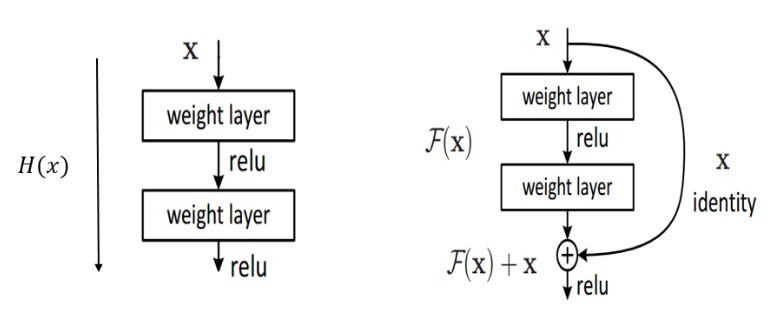
\includegraphics[width=0.5\textwidth]{figures/ResidualBlock.jpg}
	\caption{Schemat funkcjonalny pojedynczego bloku w architekturze ResNet.}
	\label{ResNetBlock}
\end{figure} 

Ogólną postać równania bloku rezydualnego można zapisać następująco:
\begin{equation}
\begin{split}
y_l = h(x_l) + F(x_l, W_l),\\
x_{l+1} = f(y_l),
\end{split}
\end{equation}
gdzie $x_l$ i $x_{l+1}$ stanowią sygnał wejściowy i wyjściowy $l$-tego bloku. $F$ stanowi funkcję rezydualną optymalizowaną podczas treningu sieci, $h$($x_l$) stanowi funkcję przekształcenia sygnału $x_l$ przekazywanego skrótowym połączeniem, $f$ jest funkcją ReLU, a $W$ stanowi macierz wag.

Funkcja $h$($x_l$) jest funkcją tożsamościową, a zatem $h$($x_l$) = $x_l$. Żeby uzasadnić ten wybór należy rozważyć propagację gradientu wewnątrz sieci skłądającej się z bloków rezydualnych. Dla każdego $L$-tego bloku zachodzi równanie:
\begin{equation}
x_L = x_l + \sum_{i=l}^{L-1}F(x_i, W_i)
\end{equation}
Korzystając z reguły łąńcuchowej [ResNet-wyj-9] można zapisać równanie na gradient funkcji kosztu $\varepsilon$:
\begin{equation}
\ref{gradResBlock}
\frac{\partial \varepsilon}{\partial x} =  \frac{\partial \varepsilon}{\partial x_L} \frac{\partial x_L}{\partial x_l} =  \frac{\partial \varepsilon}{\partial x_L}\left (1 +   \frac{\partial }{\partial x_l}\sum_{i=l}^{L-1}F(x_i, W_i) \right )
\end{equation}
z czego wynika, że gradient może być podzielony na dwie addytywne składowe: (1) $w$ = $\frac{\partial \varepsilon}{\partial x_L}$ propagowaną bez wpływu na warstwy zawierające wagi i (2) $\lambda$ = $\frac{\partial \varepsilon}{\partial x_L}\frac{\partial }{\partial x_l}\sum_{i=l}^{L-1}F(x_i, W_i)$ propagowaną przez nie.

Przykład propagacji gradientu w sieci składającej się z trzech bloków wyglądałby następująco:
\begin{equation}
\frac{\partial \varepsilon}{\partial x_0} =  \frac{\partial \varepsilon}{\partial x_3}*(w_2+\lambda_2)*(w_1+\lambda_1)*(w_0+\lambda_0)
\end{equation}

Przyjmując, że wartości $w$ są zazwyczaj znormalizowane do przedziału (-1;1) można rozważyć 4 istotne przypadki:
\begin{enumerate}
	\item $\lambda$ = 0 -- nie ma skrótowych połączeń, co odpowiada płaskiej strukturze sieci. Ponieważ wartości $w$ są z przedziału (-1;1) dodawanie kolejnych warstw wzmacnia wcześniej omówiony efekt zanikającego gradietu.
	\item $\lambda$ $>$ 1 -- z każdą warstwą, sumaryczna wartość gradientu zwiększa się inkrementalnie, co nazywane jest \textit{problemem eksplozji gradientu} (ang. \textit{exploding gradient problem}).
	\item $\lambda$ $<$ 1 -- przy założeniu, że $w$ + $\lambda$ $<$ 1, dla sieci skłądających się z wielu warstw występuje problem zaniku gradientu, jak w przypadku 1. Natomiast, gdy $w$ + $\lambda$ $>$ 1 podobnie jak w przypadku 2 może występować problem eksplozji gradienu.
	\item $\lambda$ $=$ 1 -- wartości $w$ są inkrementowane dokładnie o 1, co eliminuje problemy podane w przypadkach 1, 2 i 3 i stanowiło motywacje dla twórców architektury ResNet dla wyboru funkcji tożsamościowej $h$($x_l$).
\end{enumerate}

Dokładny opis matematyczny funkcjonowania bloków rezydualnych wraz z dowodami znajduje się w [ResNet-wyj]. Przykład topologii sieci składającej się z 8 bloków i łącznie 18 warstw tzw. ResNet-18, przedstawiono na Rys.
\begin{figure}[h!]
	\centering
	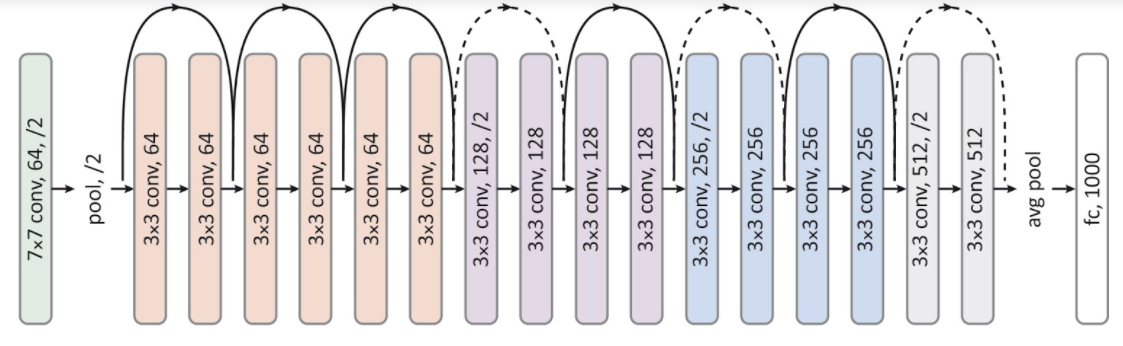
\includegraphics[width=1\textwidth]{figures/ResNet.png}
	\caption{Topologia architektury ResNet-18.}
	\label{ResNetBlock}
\end{figure} 

Pierwsza warstwa konwolucyjna zawiera filtry z jądrem splotu o wymiarach 7$\times$7. W kolejnych zastosowano wymiar 3$\times$3. Zastosowanie mniejszych wymiarów jąder splotu niż w AlexNet oraz podobnie jak w przypadku sieci GoogLeNet wyliczenie na końcu wartości średniej z dwuwymiarowych map cech zredukowało liczbę parametrów.

Architektura ResNet-18 jest najmniejszą z pojawiających się w literaturze przykładów. W praktyce, z powodzeniem wykorzystywano topologie składające się nawet z 1202 warstw [ResNet]. W 2016 roku zaprezentowano hybrydę sieci GoogleNet i ResNet [InceptionResNet]. Pracowano również nad bardziej złożonymi blokami, co w konsekwencji doporwadziło w 2017 roku do zaprezentowania architektury ResNetX, która w wielu testach klasyfikacji różnych zbiorów okazała się być lepsza niż poprzednicy [ResNetX]. Ciekawy przegląd dotyczący historii tych prac można znaleźć w [https://towardsdatascience.com/an-overview-of-resnet-and-its-variants-5281e2f56035].

Sieć ResNet i jej warianty dla wielu testowych zbiorów danych takich jak ImageNet, CIFAR czy COCO osiągneły dokładność klasyfikacji porównywalną z możliwościami ludzkiego obserwatora. Dalszy progres był możliwy m.in. dzięki zastosowaniu synergii wielu modeli, co zostało opisane w kolejnej podsekcji.

\subsection{Złożenia}
Uczenie złożeń sieci (ang. \textit{esemble learning}) polega na wykorzystywaniu kilku modeli bazowych i wybranej metody ich synergii. Koncepcja nie jest nowa i stosowana była już przed etapem kiedy to metody głębokiego uczenia się zyskały na popularności. Dobry przegląd wcześniejszych prac bazujących na tradycyjnym podejściu do uczenia maszynowego można znaleźć w  [Ensemble 1-3].

W kontekście głębokiego uczenia się stosowane są różnea metody kombinacji modeli bazowych [Ensemble]. Jako często stosowane przykłady można podać: uśrednianie, głosowanie, klasyfikacja Bayesa, generalizację stosów. Zostaną one omówione w kolejnych paragrafach:

\subsubsection{Uśrednianie}
Uśrednianie jest prostą metodą kombinacji wyników predykcji. Najczęściej stosowane jest uśrednianie bez wag, gdzie suma wyników predykcji modeli bazowych podzielona jest przez liczbę tych modeli. Uśredniać można bezpośrednio wyniki finalnej predykcji jak również prawdopodobieństwa przynależności do odpowiednich klas, które są np. wynikiem funkcji softmax. 

Główną zaletą uśredniania jest redukcja wariancji. Jest ona tym większa im bardziej nieskorelowane są wyniki predykcji modeli bazowych. Pomimo prostoty tego rodzaju koncepcja odnosiła już sukcesy m.in. w lasach losowych (Breiman, 2001).

Zastosowanie uśredniania przy silnie odstających od średniej najgorszych predykcjach znacząco obniża dokładność całego złożenia. Dlatego przy silnie nieheterogenicznych modelach bazowych dających bardzo różne wyniki często poszukiwane są inne metody.

\subsubsection{Głosowanie}

W głosowaniu stosuje się mechanizm zliczania przewidzianych przez modele bazowe etykiet. Etykieta, która została wybrana przez największą liczbę modeli bazowych jest obierana jako wynik ostatecznej predykcji. Jest to tzw. \textit{głosowanie większościowe}.

W porównaniu do uśredniania, głosowanie jest mniej czułe na predykcje pojedynczych modeli. Wykorzystuje jednak jedynie informacje o przewidzianych etykietach, co utrudnia konstrukcje bardziej wyszukanych rozwiązań.

\subsubsection{Klasyfikacja Bayesa}

W przypadku tej metody, każdy model bazowy $j$ postrzegany jest jako hipoteza $h_j$. Każda z hipotez posiada wagę proporcjonalną do prawdopodobieństwa zdarzenia, w którym dany zbiór danych trenujących zostałby wybrany z ogółu danych gdyby dana hipoteza była prawdziwa. Jest to tzw. optymalna klasyfikacja Bayesa, którą można zapisać następującycm równaniem:
\begin{equation}
y = armax_{c_j \in C} \sum_{h_i \in H} P(c_j \mid h_i)P(T \mid h_i)P(h_i)
\end{equation}
gdzie $y$ to przewidziana etykieta, $C$ jest zbiorem wszystkich możliwych klas, $H$ to przestrzeń hipotez, a $T$ to zbiór danych trenujących.

W praktyce z uwagi na dużą złożoność obliczeniową optymalną klasyfikację Bayesa wykorzystuje się rzadko. Cześćiej stosowane są techniki BPA (od ang. \textit{Bayesian parameter averaging}), BMA (od ang. \textit{Bayesian model averaging}), czy teć BMC (od ang. \textit{Bayesian model combination}) (zob. [BPA, BMA, BMC]), które aproksymują optymalną metodę.

\subsubsection{Generalizacja stosów}
Idea generalizacji stosów oryginalnie została zaproponowana w [Wolpert, 1992]. Wykorzystana została koncepcja meta-uczenia, a zatem konstrukcja nadrzędnego klasyfikatora, którego zadniem jest wybór optymalnego wektora wag $a$ dla stosu $s$ predykcji dla danych $x$:
\begin{equation}
s(x) = \sum_{i=1}^{m}a_i s_i(x)
\end{equation}

W praktyce predykcje z modeli bazowych składowane są na stosie, a następnie klasyfikator nadrzędny wykorzystuje je jako dane do swojego treningu poprawnych wartości $a$ wykorzystując jako odniesienie znane, poprawne etykiety.
 

\section{Zastosowania w medycynie}

W 1994 roku ukazała się pierwsza praca, która w praktyce wykorzystywała mechanizmy związane z głębokim uczeniem do przetwarzania obrazów medycznych [Zhang, 1994]. Użyte wówczas sieci nazywano sieciami typu \textit{shift-invariant}. Zastosowanie ich pozwoliło na eliminacje 55\% FP otrzymywanych przy wcześniejszych metodach stosowanych do detekcji skupisk mikrozwapnień w mommografach. \textit{Shift-invariant} oznaczało, że przesunięcie obrazu wejściowego nie powodowało zmian w klasyfikacji, co jest istotną cechą z uwagi na implementację toru akwizycji danych w praktyce radiologicznej.

Po roku 2012 nastąpił znaczący wzrost zainteresowania metodami głębokiego uczenia się w medycynie. Obrazuje to praca z 2017, w której przytoczono statystyki medycznych publikacje zawierających słowa kluczowe związane z głębokim uczeniem się [arXiv:1702.05747v2]. Najważniejsze dane przedstawiono a Rys. \ref{DL_CAD_stats}.
\begin{figure}[h!]
	\centering
	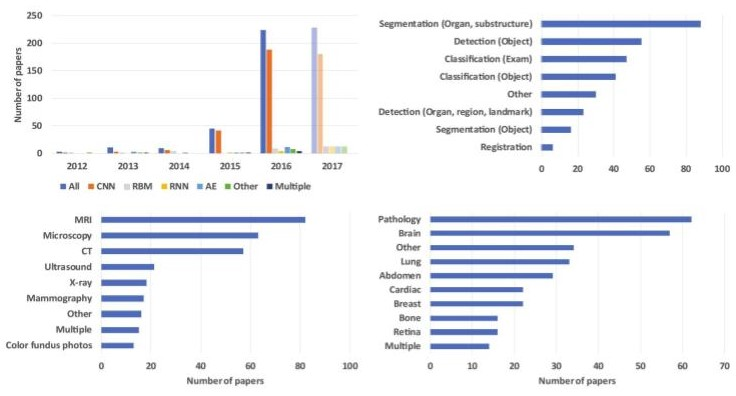
\includegraphics[width=1\textwidth]{figures/DL_CAD_statystyka.jpg}
	\caption{Statystyki dotyczące publikacji medycznych zawierających słowa kluczowe związane z głębokim uczeniem się.}
	\label{DL_CAD_stats}
\end{figure}

 Widoczny wzrost liczby publikacji nastąpił począwszy od 2015, co związane było z kilkuletnią adaptacją nowych metod w dziedzinie przetwarzania obrazów medycznych i gromadzeniem odpowiednich danych. Rok 2016 i 2017 były pod pewnym względem przełomowe gdyż pojawiało się coraz więcej prac naukowych, w których przedstawiano rezultaty dokładności klasyfikacji medycznych zbiorów danych na poziomie dorównującym ekspertom dziedzinowym.
 
 Dla przykładu, w Listopadzie 2016 ukazał się praca grupy Google Research, Mountain View, Kalifornia [https://www.ncbi.nlm.nih.gov/pubmed/27898976], gdzie zastosowano sieć GoogLeNet w wersi inception-v3 do zautomatyzowanej detekcji retinopatii cukrzycowej i cukrzycowego obrzęku plamki w obrazach dna oka. Wyniki porównano z panelem skjładającym się z 7 ekspertów, okulistów. Porównanie przedstawiono na Rys. \ref{CAD_opto}.
 \begin{figure}[h!]
 	\centering
 	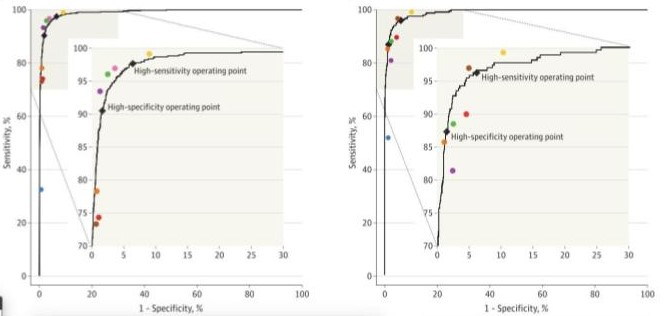
\includegraphics[width=0.7\textwidth]{figures/CAD-okulisci.jpg}
 	\caption{Porównanie automatycznej klasyfikacji retinopatii cukrzycowej i cukrzycowego obrzęku plamki z oceną panelu ekspertów}
 	\label{CAD_opto}
 \end{figure}
 
 Na wykresach dla dwóch zadań klasyfikacyjnych umieszczono krzywe reprezentujące zależność swoistości od czułości dla algorytmu automatycznego oraz 7 punktów oznaczające wynik oceny każdego z ekspertów-okulistów. Ogółem mniej niż połowa ekspertów uzyskałą lepszy wynik niż algorytm sztucznej inteligencji.
 
 Kolejna ciekawa praca pojawiła się w czasopiśmie nature w styczniu 2017 i traktowała o automatycznej detekcji raka skóry na zdjęciach [Esteva, 2017]. Autorzy wykorzystali dane składające się z 129,450 obrazów klinicznych, na których zobrazowano 2,032 różne schorzenia skóry. Ponownie do klasyfikacji wykorzystano sieć GoogleNet w wersji inception-v3. Wyniki klasyfikacji automatycznej porównano z oceną przeprowadzoną przez 21 certyfikowanych dermatologów. Przykład porównania zaprezentowano na Rys. \ref{CAD_derma}. 
 
 \begin{figure}[h!]
 	\centering
 	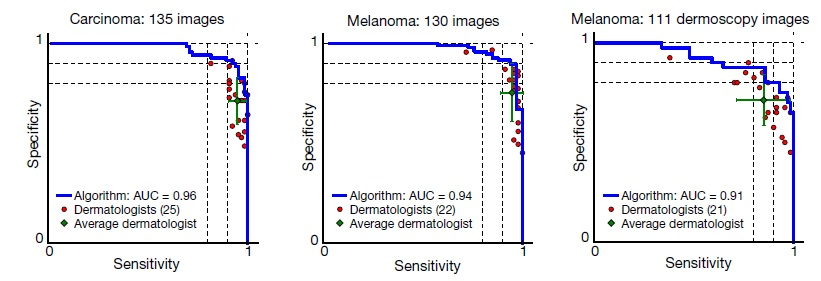
\includegraphics[width=0.9\textwidth]{figures/CAD-dermatolodzy.jpg}
 	\caption{Porównanie automatycznej klasyfikacji 3 chorób skóry z oceną ekspertów dermatologów}
 	\label{CAD_derma}
 \end{figure}

Tym razem umieszczono odwrotną zależność (tj. czułość od swoistości), czerwonymi punktami oznaczono wynik oceny ekspertów, a zielonym krzyżykiem wynik uśrednienia oceny eksperckiej. W każdym przypadku średnia ocena była gorsza od automatycznje klasyfikacji.

Ostatni przykład zaprezentowany w tej pracy został opublikowany przez grupę ze Stanford University w 2017 roku w Lipcu i dotyczył klasyfikacji arytmii [Rajpurkar, 2017].

 Jak już wspomniano problemy w wykorzystaniu metod głębokiego uczenia się w medycynie wywodzą się z konieczności zgromadzenia dużych zbiorów, dobrze oznaczonych danych. Wymaga to bliskiej współpracy ekspertów medycznych (najczęściej radiologów) z ekspertami od uczenia maszynowego oraz modyfikacja bądź tworzenie dedykowanych programów do akwizycji danych medycznych. Jako przykłady takich synergii można wymienić programy Stanford Medicine [MedicalImageNet], Harward School of Medicine [10 mln images] czy Masachuset Hospital [NVIDIA 2018]. W roku 2018 na konferencji NVIDIA GTC w San Jose (Kalifornia) Amerykańskie Stowarzyszenie Radiologii i stowarzyszenie MICCAI (od ang. \textit{Medical Image Computing and Computer Assisted Intervention}) ogłosiły porozumienie, co do wspólnej współpracy mającej na celu eliminacje barier legislacyjnych związanych ze współpracą przy pozyskiwaniu odpowiednich danych dla wykorzystania algorytmów uczenia maszynowego.
 
    
